\subsection{4.6液晶聚合物}

液晶聚合物(液晶聚合物)是含有棒状“液晶”基元的高分子材料,能够在流体-即所谓的液晶状态下产生自发定向秩序。液晶的性质可以有很大不同,这取决于液晶基元的形状和化学细节。向列相、近晶相和胆甾相是最常见的液晶有序情况,但可以找到更复杂的例子,甚至在低分子量液晶中也是如此。德热纳(de Gennes)和普罗斯特(Prost)(1993)的专著对液晶流体的物理学作了很好的介绍。\\

1.\textbf{无序相.}无序相是指空间位置和指向都无序(服从均匀分布)的结构.热致液晶在高温或者溶致液晶在低密度时容易形成无序相;\\

2.\textbf{向列相.}向列相是指空间位置无序、指向有序(所有分子的指向接近平行)的结构;\\
\begin{figure}[H]
	\centering   
	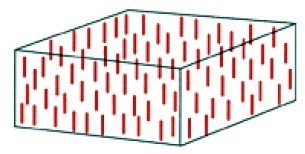
\includegraphics[width=12cm]{./figures/4.png}
	%\caption{向列相}
\end{figure}
3.\textbf{近晶相.}近晶相是空间和指向都有序的一种微观结构. 与晶体类似,近晶相的空间排列有序,故而称为近晶相,该相是由液晶棒状分子聚集一起,形成一层一层的周期结构,每一层的分子的长轴方向相互平行;\\
\begin{figure}[H]
	\centering   
	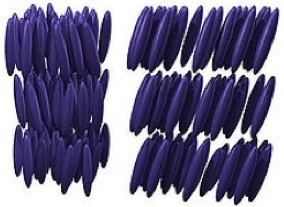
\includegraphics[width=12cm]{./figures/3.png}
	%\caption{近晶相}
\end{figure}
4.\textbf{胆甾相.}此类液晶分子呈扁平状,排列成层,层内分子相互平行,分子长轴平行于层平面,不同层的分子长轴方向稍有变化,沿层的法线方向排列成螺旋状结构。\\
\begin{figure}[H]
	\centering   
	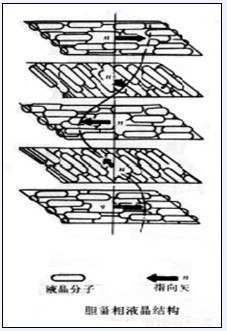
\includegraphics[width=12cm]{./figures/5.png}
	%\caption{胆甾相}
\end{figure}

当液晶基元被结合到聚合物中时,呈现定向有序相的可能性显著增强。中间基元可以以均匀的方式结合到主链中,也可以连接到侧链上,分别产生主链液晶聚合物或侧链液晶聚合物。 第二种广义分类是指液晶的顺序通过温度(如所谓的热带)或溶液中聚合物浓度的改变而改变,在这种情况下,液体是热带流体。通过随机共聚合或嵌段/接枝共聚,中间元也可以作为主链或侧链单元并入大分子中。体系结构的复杂性会导致各种现象的发生,其中定向顺序与组合顺序竞争,例如宏相分离或微相分离。\\

由于液晶聚合物代表了一组多样的材料,因此在这一范围的专著中不可能提出一套涵盖所有类型的液晶聚合物系统的全面模型。因此,我们把重点放在一个简单的代表模型主链均聚物系统上,可以显示向列序。模型$G$可以看作是一个热致,主链液晶聚合物熔体的模型,也可以看作是半柔性聚合物溶致溶液的模型。\\


\textbf{4.6.1模型G:聚合物分子动力学}

模型$G$是模型$A$的推广,但这里用蠕虫链模型代替了连续高斯链,并加入了聚合物段间的各向异性相互作用。主链向列型聚合物往往是半柔性的,因为液晶元结合在他们的脊骨。应用蠕虫链模型,默认弯曲阻力沿链是均匀的。对于许多类型的主链液晶聚合物来说,这种假设显然是不现实的,但它为理解聚合物的行为提供了一个简单的起点。\\

为了表示各向异性相互作用导致的向列序,将片段位置和取向的微观密度的定义$(3.35)$推广到含有$n$个蠕虫状聚合物的体系中:\\
\begin{equation}
\hat{\rho}(\br,\bu) \equiv \sum_{j=1}^{n} \int _{0}^{L_{c}} \delta(\br-\br_{j}(s)) \delta (\bu-\bu_{j}(s))~ds
\end{equation}

如果我们引用相互作用势的近似,在$\hat{\rho}(\br,\bu)$中,段间非键相互作用对势能的贡献可以描述为二次型:\\
\begin{equation}
U_1=\frac{1}{2} \int d\br \int d\br' \int d\bu \int  \hat{\rho}(\br,\bu) \upsilon_2(\br,\br',\bu,\bu') \hat{\rho}(\br',\bu')~d\bu'
\end{equation}
其中$\upsilon_2$是一个合适的对势函数,假定它在接触时被正则化。我们还了解到,在溶致体系中,$\upsilon_2$为平均力的对势,并取决于纯溶剂的性质。\\

在液晶聚合物系统的介观描述中,一个典型的进一步逼近是假定在空间上的相互作用是局部的,这相当于$\upsilon_2$的$\delta$函数近似:\\
\begin{equation}
\upsilon_{2}(\br,\br',\bu,\bu') \approx \delta(\br-\br') \upsilon(\bu,\bu')
\end{equation}
其中$\upsilon(\bu,\bu')$是与局部方向相关的相互作用。$\upsilon$的形式不是任意的,它是对称的,并且对于$\bu,\bu'$的符号反转都是不变的。$\upsilon$的常见表达式是昂萨格(Onsager)形式\\
\begin{equation}
\beta \upsilon(\bu,\bu')= u_{1}|\bu\times \bu'|
\end{equation}

它来源于昂萨格的溶致液晶聚合物理论和$Maier-Saupe$(Maier-Saupe)形式。\\
\begin{equation}
\beta \upsilon(\bu,\bu')=u_0 - u_{2} P_{2}(\bu \cdot \bu')
\end{equation}

这是热致液晶的$Maier-Saupe$理论的基础。昂萨格形式产生于两个方向为$\bu$和$\bu'$的细长棒之间排除体积的计算,并导致与温度无关(非热)微观长度的预因子$u_{1}>0$。 $Maier-Saupe$形式包含各向同性排除体积项$u_{0}>0$,类似于$(4.62)$,以及一个与$u_2>0$成正比的各向异性四次项。后者乘$P_{2}(\bu,\bu')\equiv (1/2)[3(\bu\cdot \bu')^2-1]$,这是$(2.84)$中定义的二阶勒让德多项式。在原始理论中,假设各向异性系数$u_2$是由范德华尔斯相互作用导出的,因此,在现实中,昂萨格和$Maier-Saupe$形式都是唯象的,因为通过拟合实验数据得到的参数$u_0$、$u_1$和$u_2$的值很少符合这些纯粹熵或纯焓期望。在这两种情况下,稳定向列序的关键是$\upsilon (\bu,\bu')$ 随着两个相邻聚合物段的相互排列而减小。\\

$n$个相互作用的蠕虫链的正则配分函数可以表示为包含上述非键段相互作用的玻尔兹曼因子$\exp (-\beta U_1)$上的$(2.67)$形式的$n$个路径积分的乘积。通过引用模型$A$中的$(4.69)$和$(4.70)$的步骤,可以将这个表达式转换为场论。我们得到以下规范模型$G$场论:\\
\begin{equation}
Z_{C}(n,V,T)=Z_{0} \int \mathcal{D} \rho \int  \exp (-H[\rho,w])~\mathcal{D} w
\end{equation}
有效哈密顿量\\ 
\begin{equation}
H[\rho,w]= -i \int d\br \int d\bu w(\br,\bu) \rho(\br,\bu)-n \ln Q[i w]+\frac{\beta}{2} \int d\br \int d\bu \int  \rho(\br,\bu) \upsilon(\bu,\bu') \rho(\br,\bu')~d\bu'
\end{equation}
其中$Q[i w]$是由$(3.36)$定义的纯虚势$i w(\br,\bu)$中单个蠕虫聚合物链的归一化配分函数。在该模型中,$Z_0$为$n$个非相互作用蠕虫状聚合物链的理想气体的配分函数。\\

在$\upsilon(\bu,\bu')$为正定且具有逆函数的情况下,可以在波动的$\rho(\br,\bu)$场上进行高斯积分,从而在单场$w(\br,\bu)$上实现更简单的场理论。不幸的是,对于昂萨格或$Maier-Saupe$形式,$\upsilon$都不是正定的,这可以很容易地通过球谐展开来验证。因此,模型$G$场理论的简化形式,类似于模型$A$的$(4.71)$和$(4.72)$,对向列相聚合物的适用性有限。\\

在全正则模型$G$场理论中,分段密度$\rho(\br,\bu)$显式出现,因此平均数、段数密度和方向矩可以直接获得。第二个重要的密度算子,只依赖于$w$场,它可以被定义为\\
\begin{equation}
\tilde{\rho}(\br,u;[i w]) \equiv -n \frac{\delta \ln Q[i w]}{\delta i w(\br,\bu)}
\end{equation}

它是$(3.62)$的单链密度算子$\rho(\br,\bu;[i w])$,乘以聚合物数$n$。由此可以从$(3.39)$和$(3.63)$的解中求出这个算子对$w$的表达式。可以根据$(3.64)-(3.67)$定义其他的简化段密度算子。\\

另一个液晶聚合物中的算子是向列序参数张量$S_{\alpha \beta}(\br;[\rho])$,该算子可以定义为\\
\begin{equation}
S_{\alpha \beta}(\br;[\rho]) \equiv \frac{V}{n L_{c}} \int \rho(\br,\bu)(u_{\alpha} u_{\beta}-\frac{1}{3} \delta_{\alpha \beta})~d\bu
\end{equation}

它对$\rho$场波动的期望值为系统中向列序的范围和空间变化提供了一种有用的度量。最后,需要指出的是,在有效哈密顿量$(4.135)$中,用$-n \ln Q$代替$-z VQ$得到了模型$G$场理论的一个巨正则版本。\\
